\section{Units of mitigation}


\subsection{Einleitung}

Dieses, wie auch die folgenden Patterns, zielen auf alle Teile eines Systems ab, und nicht nur auf ein bestimmtes Modul oder eine bestimmte Klasse.

Die Architektur eines Systems hat einen beträchtlichen Einfluss auf die Fehlertoleranz. Deshalb sind die Architectural Patterns auch die ersten, die auf ein neues Projektdesign angewendet werden und sind aus diesem Grund auch die ersten in diesem Buch beschriebenen.

\begin{figure}[H]
	\centering
	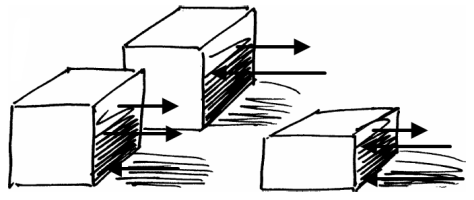
\includegraphics[width=\textwidth]{content/faulttolerance/images/unitsOfMitigation.png}
	\caption{unitsOfMitigation}
\end{figure}


\subsection{Problem}

Wie kann ich verhindern, dass das ganze System ausfällt, sobald irgendwo ein Fehler auftritt? Es sollte möglich sein, dass nur ein Teil ausfällt, den Fehler bestenfalls behebt und sich dann wieder ins System einklinkt.

Dieser eine Teil wird hier 'unit of mitigation' genannt. Wieviele davon das System enthält, und wie gross diese sind, hängt sehr von der jeweiligen Situation ab.

Wie alle Massnahmen zur Fehlertoleranz liefert auch die unit of mitigation ('Einheit zur Schadensmilderung') einen overhead an Code und Komplexität. Sie sollte deshalb nicht zu klein gewählt werden (beispielsweise jeden Ort 'einkapseln', an dem ein Fehler auftreten kann).
Ist sie zu gross, sind wir wieder beim Beispiel, dass das ganze System ausfällt. Es gilt also, einen guten Mittelweg zu finden.

\subsection{Lösung}

\textbf{\textit{Teile das System so ein, dass jeder Teil sowohl mögliche Fehlerquellen wie auch Massnahmen zur Erkennung und Behebung beinhaltet.}} Wähle die Aufteilung so, dass sie für dein System Sinn macht.

Als mögliche, natürliche Trennlinien können in Frage kommen:
\begin{itemize}
	\item Tiers / Layers
	\item Teilapplikationen
	\item Prozessoren, Cores
	\item Threads
	\item Tasks
	\item Terminals / Protokol Handlers
	\item Gruppen von Funktionalitäten
\end{itemize}

Die units of mitigation sollten gegen Aussen genau definierte Interfaces haben. Diese bilden dann eine strikte Barriere für die Fehler und es sollte höchstens bekannt gegeben werden, dass ein solcher aufgetreten ist. Dies bedingt, dass eine Einheit in der Lage sein muss, Fehler zu erkennen und zu beheben.

Das Hinzufügen von Redundanz kann helfen, das System lauffähig zu halten. Ist eine unit damit beschäftigt, einen Fehler zu beheben, kann das redundante Gegenstück einspringen und die Mehrarbeit übernehmen.

Lässt sich ein Modul gut restarten, spricht dies für eine gute Wahl einer unit of mitigation.


